\RequirePackage{plautopatch}
\documentclass[11pt,aspectratio=169,xcolor=dvipsnames,table,dvipdfmx]{beamer}
\usepackage{bxdpx-beamer} % dvipdfmxなので必要
\usepackage{appendixnumberbeamer}

%Beamerの設定
\usetheme{Boadilla}

%Beamerフォント設定
\usefonttheme{professionalfonts} % Be professional!
\usepackage[T1]{fontenc}
\usepackage{mlmodern}  % 太いComputer Modern
% MLmodernのバグを修正: cf. https://tex.stackexchange.com/questions/646333/size-of-integral-symbol-in-section-header-with-mlmodern
\DeclareFontFamily{OMX}{mlmex}{}
\DeclareFontShape{OMX}{mlmex}{m}{n}{%
   <->mlmex10%
   }{} 
\usepackage{newtxtext} % 数式以外をTXフォントで上書き
\usepackage[deluxe,uplatex]{otf} % 日本語多ウェイト化
\usepackage{physics,bm}
\usepackage{mhchem}
\usepackage{amsmath,amsfonts,amssymb,mathtools,amsthm}
\DeclareMathOperator{\sgn}{sgn}
\renewcommand{\familydefault}{\sfdefault}  % 英文をサンセリフ体に
\renewcommand{\kanjifamilydefault}{\gtdefault}  % 日本語をゴシック体に
\usefonttheme{structurebold} % タイトル部を太字
\setbeamerfont{alerted text}{series=\bfseries} % Alertを太字
\setbeamerfont{section in toc}{series=\mdseries} % 目次は太字にしない
\setbeamerfont{frametitle}{size=\Large} % フレームタイトル文字サイズ
\setbeamerfont{title}{size=\LARGE} % タイトル文字サイズ
\setbeamerfont{date}{size=\small}  % 日付文字サイズ

% Babel (日本語の場合のみ・英語の場合は不要)
\uselanguage{japanese}
\languagepath{japanese}
\deftranslation[to=japanese]{Theorem}{定理}
\deftranslation[to=japanese]{Lemma}{補題}
\deftranslation[to=japanese]{Example}{例}
\deftranslation[to=japanese]{Examples}{例}
\deftranslation[to=japanese]{Definition}{定義}
\deftranslation[to=japanese]{Definitions}{定義}
\deftranslation[to=japanese]{Problem}{問題}
\deftranslation[to=japanese]{Solution}{解}
\deftranslation[to=japanese]{Fact}{事実}
\deftranslation[to=japanese]{Proof}{証明}
\def\proofname{証明}

%Beamer色設定
\definecolor{UniBlue}{RGB}{0,150,200} 
\definecolor{AlertOrange}{RGB}{255,76,0}
\definecolor{AlmostBlack}{RGB}{38,38,38}
\setbeamercolor{normal text}{fg=AlmostBlack}  % 本文カラー
\setbeamercolor{structure}{fg=UniBlue} % 見出しカラー
\setbeamercolor{block title}{fg=UniBlue!50!black} % ブロック部分タイトルカラー
\setbeamercolor{alerted text}{fg=AlertOrange} % \alert 文字カラー
\mode<beamer>{
    \definecolor{BackGroundGray}{RGB}{254,254,254}
    \setbeamercolor{background canvas}{bg=BackGroundGray} % スライドモードのみ背景をわずかにグレーにする
}

%フラットデザイン化
\setbeamertemplate{blocks}[rounded] % Blockの影を消す
\useinnertheme{circles} % 箇条書きをシンプルに
\setbeamertemplate{navigation symbols}{} % ナビゲーションシンボルを消す
\setbeamertemplate{footline}[frame number] % フッターはスライド番号のみ
\setbeamerfont{footline}{size=\small}    % フッターを大きくした

%タイトルページ
\setbeamertemplate{title page}{%
    \vspace{2.5em}
    {\usebeamerfont{title} \usebeamercolor[fg]{title} \inserttitle \par}
    {\usebeamerfont{subtitle}\usebeamercolor[fg]{subtitle}\insertsubtitle \par}
    \vspace{1.5em}
    \begin{flushright}
        \usebeamerfont{author}\insertauthor\par
        \usebeamerfont{institute}\insertinstitute \par
        \vspace{3em}
        \usebeamerfont{date}\insertdate\par
      \end{flushright}
      \vspace{-6em}
      \begin{flushleft}
        \usebeamercolor[fg]{titlegraphic}\inserttitlegraphic
      \end{flushleft}
}

% Algorithm系
\usepackage{algorithm}
\usepackage[noend]{algorithmic}
\algsetup{linenosize=\color{fg!50}\footnotesize}
\renewcommand\algorithmicdo{:}
\renewcommand\algorithmicthen{:}
\renewcommand\algorithmicrequire{\textbf{Input:}}
\renewcommand\algorithmicensure{\textbf{Output:}}

% 定理
\theoremstyle{definition}
\newenvironment{mythm}{\begin{alertblock}{定理}}{\end{alertblock}} %自分の結果は赤色で表示

\AtBeginSection[]{
    \frame{\tableofcontents[currentsection, hideallsubsections]} %目次スライド
}
\usepackage[absolute,overlay]{textpos}
\usepackage{array} % needed for \arraybackslash
\usepackage{adjustbox} % for \adjincludegraphics

\usepackage{tikz}
\usetikzlibrary{calc}
\makeatletter
\chardef\zenkakuSpace=\jis"2121\relax % 和文ゴースト用全角スペース

\def\serifRoman#1{%
  \ifnum0\ifnum#1<1 1\fi\ifnum#1>12 1\fi>0 %%% 引数が 1~12 の範囲外ならエラー
    \@latex@error{\string\serifRoman: #1 must be 1..12}\@ehc
  \fi
  \zenkakuSpace\kern-1zw\relax %%% ゴースト処理(入口側)
  \begingroup
  \@tempcnta="215F\relax
  \advance\@tempcnta by #1\relax
  \kchardef\@roman@char=\ucs\@tempcnta\relax %% 今回対象のローマ数字
  \kchardef\@roman@I=\ucs"2160\relax %% ヒゲとして利用するローマ数字Ⅰ
  \@tempdima=-.132zw\relax
  \@tempdimb=.134zw\relax
  \@tempdimc=1zw\relax
  \setbox1\hbox to 1zw{\yoko\hfill
    \begin{tikzpicture}[baseline=(A.base),inner sep=0pt, outer sep=0pt]%
    \path[use as bounding box] (-.5\@tempdimc, -.5\@tempdimc) rectangle (.5\@tempdimc, .5\@tempdimc);
    \node (A) {\@roman@char};
    \ifcase#1
      \or % Ⅰ
        \@serifRoman@a{.45}{0}% 上ヒゲ
        \@serifRoman@b{.45}{0}% 下ヒゲ
      \or % Ⅱ
        \@serifRoman@a{.80}{0}% 上ヒゲ
        \@serifRoman@b{.80}{0}% 下ヒゲ
      \or % Ⅲ
        \@serifRoman@a{1.10}{0}% 上ヒゲ
        \@serifRoman@b{1.10}{0}% 下ヒゲ
      \or % Ⅳ
        \@serifRoman@a{.60}{-.24}% 左上ヒゲ
        \@serifRoman@a{.30}{.38}%% 右上ヒゲ
        \@serifRoman@b{.30}{-.35}% 左下ヒゲ
      \or % Ⅴ
        \@serifRoman@a{.30}{-.28}% 左上ヒゲ
        \@serifRoman@a{.30}{.28}%% 右上ヒゲ
      \or % Ⅵ
        \@serifRoman@a{.30}{-.38}% 左上ヒゲ
        \@serifRoman@a{.60}{.24}%% 右上ヒゲ
        \@serifRoman@b{.30}{.34}%% 右下ヒゲ
      \or % Ⅶ
        \@serifRoman@a{.30}{-.41}% 左上ヒゲ
        \@serifRoman@a{.75}{.20}%% 右上ヒゲ
        \@serifRoman@b{.52}{.28}%% 右下ヒゲ
      \or % Ⅷ
        \@serifRoman@a{.30}{-.41}% 左上ヒゲ
        \@serifRoman@a{.82}{.18}%% 右上ヒゲ
        \@serifRoman@b{.65}{.245}% 右下ヒゲ
      \or % Ⅸ
        \@serifRoman@a{.25}{.33}%% 右上ヒゲ
        \@serifRoman@a{.55}{-.22}% 左上ヒゲ
        \@serifRoman@b{.55}{-.22}% 左下ヒゲ
        \@serifRoman@b{.25}{.36}%% 右下ヒゲ
      \or % Ⅹ
        \@serifRoman@a{.25}{.23}%% 右上ヒゲ
        \@serifRoman@a{.25}{-.23}% 左上ヒゲ
        \@serifRoman@b{.25}{-.26}% 左下ヒゲ
        \@serifRoman@b{.25}{.26}%% 右下ヒゲ
      \or % Ⅺ
        \@serifRoman@a{.55}{.23}%% 右上ヒゲ
        \@serifRoman@a{.25}{-.34}% 左上ヒゲ
        \@serifRoman@b{.25}{-.36}% 左下ヒゲ
        \@serifRoman@b{.55}{.23}%% 右下ヒゲ
      \or % Ⅻ
        \@serifRoman@a{.75}{.20}%% 右上ヒゲ
        \@serifRoman@a{.25}{-.38}% 左上ヒゲ
        \@serifRoman@b{.25}{-.40}% 左下ヒゲ
        \@serifRoman@b{.75}{.20}%% 右下ヒゲ
    \fi
    \end{tikzpicture}%
    \hfill}%
  \box1\relax
  \endgroup
  \kern-1zw\relax\zenkakuSpace %%% ゴースト処理(出口側)
}
\def\@serifRoman@a#1#2{%
  \node[rotate=90,xscale=.7,yscale=#1] at ($(A.north) + (#2\@tempdimc,\@tempdima)$) {\@roman@I};
}
\def\@serifRoman@b#1#2{%
  \node[rotate=90,xscale=.7,yscale=#1] at ($(A.south) + (#2\@tempdimc,\@tempdimb)$) {\@roman@I};
}
\makeatother


%タイトル
\title{軸対称Skyrme TDHFを用いた\\トンネル確率の計算}
\author{\textbf{松本侑真}}
\date{\today}
\institute{原子核理論 関澤研究室}
\titlegraphic{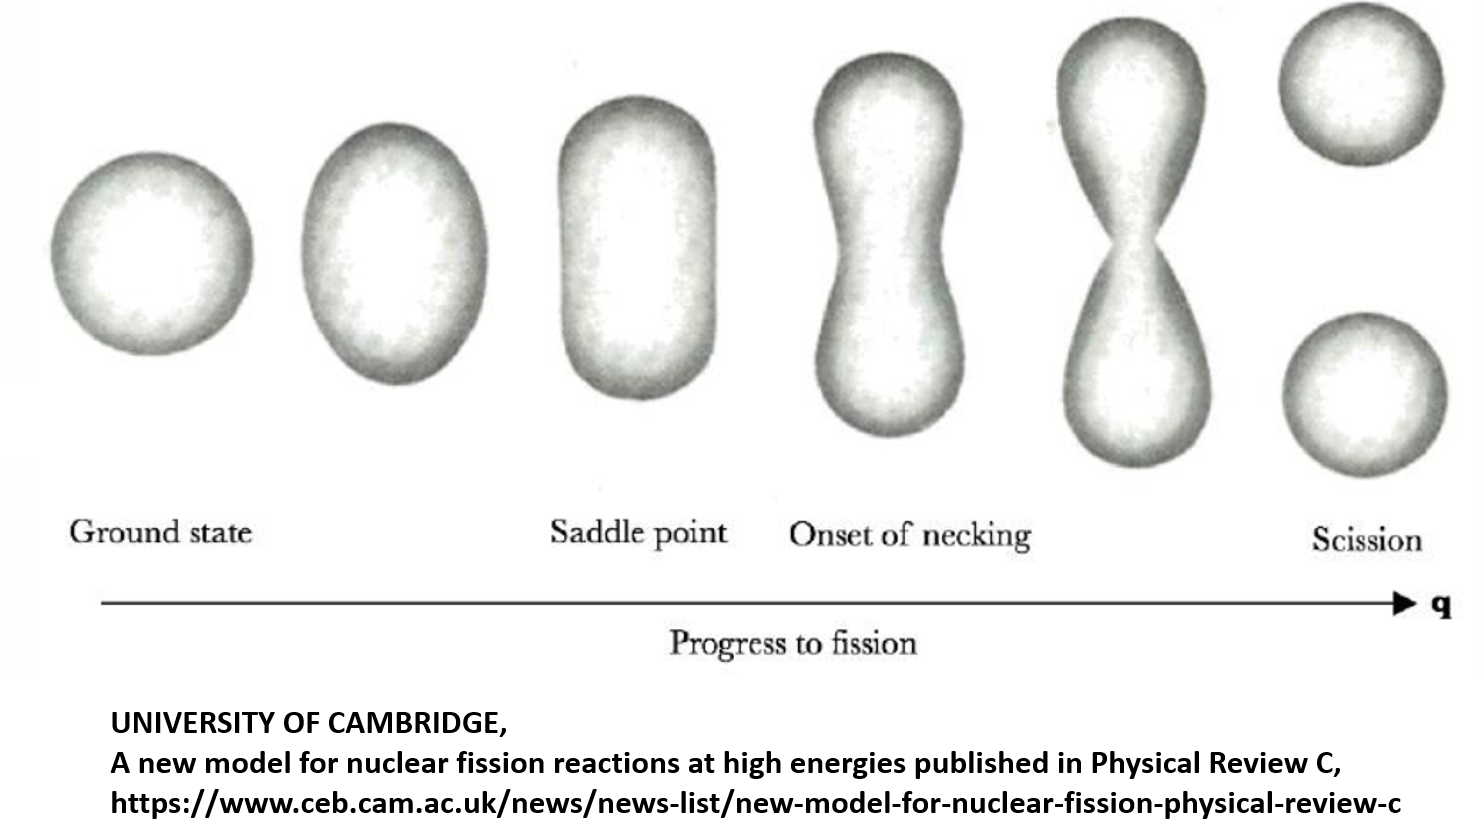
\includegraphics[scale=0.25]{fission_1.png}}
%\titlegraphic{\adjincludegraphics[height=.5\linewidth,valign=t]{heikinba.png}}

\begin{document}
\maketitle
%\frame{\tableofcontents[hideallsubsections]}

\begin{frame}
  \frametitle{研究概要}
  \begin{itemize}
    \item 3次元空間で軸対称性を課した原子核において、平均場理論に基づいた原子核の基底状態を求める自作プログラムを作成する。
    \item 完成したプログラムを用いて、実時間発展ではトンネル効果を再現できないことを確認する。
    \item 虚時間発展を組み込んで、平均場理論の枠組みでトンネル確率を計算することを目指す。
  \end{itemize}
\end{frame}


\begin{frame}{背景}
  \begin{columns}[t]
    \begin{column}{.5\textwidth}
      \begin{itemize}
        \item トンネル効果によって生じる現象が存在する
        \item 1次元模型では、ガモフによる$\alpha$崩壊の理論やWKB近似などがある
        \item 実際の核分裂は多粒子系のトンネル現象かつ複雑な形状の自由度があり、微視的な計算が困難
      \end{itemize}
      \vskip\baselineskip
      \begin{itemize}
        \item \textbf{本研究の目的:} 平均場理論に虚時間法を適用し、核子自由度から微視的に多体のトンネル現象を記述すること
      \end{itemize}
  
    \end{column}
    \begin{column}{.5\textwidth}
      \adjincludegraphics[height=1\linewidth,valign=t]{tunneling.png}
    \end{column}
  \end{columns}

\end{frame}


\begin{frame}{背景}
  J.W.Negele, Nuclear Mean-Field Theory, Physics Today 38, 24(1985)では
  \begin{itemize}
    \item 平均場理論+虚時間法の経路積分を用いて、1粒子系のトンネル現象でWKB近似の結果を再現
    \item 少数核子系(\ce{^{8}Be})の$\alpha$崩壊の計算に応用
  \end{itemize}
  を行っている。しかし、結果の定量的な評価はしておらず、詳細は述べられていない。
  \adjincludegraphics[width=1\linewidth,valign=t]{Be.png}
\end{frame}

\begin{frame}{背景}
  P. McGlynn and C. Simenel, Phys. Rev. C 102, 064614 (2018)では
  \begin{itemize}
    \item Toy model(1次元の二重井戸モデル)において、$L\to R$へのトンネル確率を虚時間法の平均場理論を用いて計算
    \begin{itemize}
      \item 2粒子系が$L$もしくは$R$の領域に束縛される場合を考えている
    \end{itemize}
    \item 実時間発展ではトンネル確率を正しく計算できないことの確認
  \end{itemize}
  を行っている。
  \begin{center}
  \adjincludegraphics[height=0.3\linewidth,valign=t]{niju-ido.png}
  \end{center}
  \begin{itemize}
    \item あとでトンネル確率の式を説明するスライドを作成する
  \end{itemize}
\end{frame}

\begin{frame}{背景}
  \begin{columns}[t]
    \begin{column}{.5\textwidth}
      \begin{itemize}
        \item 実時間発展(上図)では、{\color{blue}厳密解}と{\color{orange}計算値}の結果が異なる
        \item 虚時間発展(下図)では、相互作用が強いほど{\color{blue}厳密解}に近づく
        \begin{itemize}
          \item $\mu$は2粒子の波動関数が同じ井戸に存在する場合の引力相互作用の強さ
        \end{itemize}
        \item 下図のような結果を\textbf{現実的な原子核系}で再現することが研究の目標である。
      \end{itemize}
    \end{column}
    \begin{column}{.5\textwidth}
      \adjincludegraphics[width=1\linewidth,valign=t]{realtime-ev.png}
      \adjincludegraphics[width=1\linewidth,valign=t]{imagtime-ev.png}
    \end{column}
  \end{columns}
\end{frame}

\begin{frame}{理論的枠組み:Hartree-Fock近似}
  \begin{itemize}
    \item Hartree-Fock(HF)近似は原子核の性質(束縛エネルギーや変形度)を上手く説明できる
    \item 時間依存のHF方程式(TDHF方程式)は核子自由度から微視的に原子核ダイナミクスを記述できる
  \end{itemize}
  \begin{block}{TDHFの問題点}
    \begin{itemize}
      \item 多体波動関数が1つのSlater行列式で表されるという近似を用いている
            \begin{itemize}
              \item 複数のSlater行列式の線形結合で波動関数を表すことで、より正確な状態が得られることが知られている
            \end{itemize}
      \item 核分裂反応のような\textbf{多体のトンネル現象を記述できない}
            \begin{itemize}
              \item 平均場が1つしかなく、核分裂していない状態と核分裂している状態の重ね合わせが記述できない
            \end{itemize}
    \end{itemize}
  \end{block}
  トンネル現象を記述するためには何らかの工夫をする必要があり、そのための手法を開発することが研究の目標である。
  \begin{itemize}
    \item 経路積分+虚時間法のことも説明する
  \end{itemize}
\end{frame}



\begin{frame}{研究手法:基底状態の求め方}
  \begin{itemize}
    \item Skyrme型の相互作用を入れたHartree-Fock(SHF)方程式を解いて原子核の基底状態を求める
  \end{itemize}
  \begin{block}{SHFの解き方}
    \begin{enumerate}
      \item 核子の一粒子波動関数(スピノル)$\psi_{\alpha}$から、
      密度
      \begin{equation}
        \rho(r,z),\,\bm{J}(r,z),\,\tau(r,\,z)
      \end{equation}を計算する。
      \item 各密度で表される平均場
      \begin{equation}
        U(r,z),\,\bm{W}(r,z),\,B(r,z)
      \end{equation}
      を計算する。
      \item 平均場で構成される一粒子ハミルトニアン$\hat{h}_{\text{q}}$を用いて、基底状態のスピノルを求める。
      \item あとでSkyrme HFの式を載せる。多分虚時間発展の前にする
      \item セルフコンシステントに解くことをいう
    \end{enumerate}
  \end{block}
\end{frame}

\begin{frame}{研究手法:基底状態の求め方}
密度や平均場が軸対称性を持つとき、核子のスピノルは以下のように表される。
\begin{equation}
  \psi_{\alpha}(\bm{r}) =
  \begin{pmatrix}
    \psi_{\alpha}^{+}(\bm{r}) \\
    \psi_{\alpha}^{-}(\bm{r})
  \end{pmatrix}
  = 
  \begin{pmatrix}
    f^{+}_{\alpha}(r,z)e^{im_{\alpha}\phi} \\
    f^{-}_{\alpha}(r,z)e^{i(m_{\alpha}+1)\phi}
  \end{pmatrix}
\end{equation}
このスピノルによって、密度は以下のように計算できる:
\begin{gather}
  \rho(r,z) = \sum_{\alpha}\qty[\abs{f_{\alpha}^{+}(\bm{r})}^2+\abs{f_{\alpha}^{-}(\bm{r})}^2],\quad 
  \bm{J}(r,z) = \sum_{\alpha}\Im[\psi_{\alpha}^{\dagger}(\bm{r})(\bm{\nabla}\cross\bm{\sigma})\psi_{\alpha}(\bm{r})],\\
  \tau(r,z) = \sum_{\alpha}\qty[\abs{\bm{\nabla}f_{\alpha}^{+}(\bm{r})}^2+\abs{\bm{\nabla}f_{\alpha}^{-}(\bm{r})}^2]\text{。}
\end{gather}
\begin{itemize}
  \item 密度が求まるとポテンシャルが求まり、一粒子ハミルトニアンが求まることをかk
\end{itemize}
\end{frame}

\begin{frame}{研究手法:基底状態の求め方}
  \begin{itemize}
    \item ここの虚時間法とトンネルの虚時間は別ものということに注意して話す
  \end{itemize}
  本プログラムでは、虚時間法によって基底状態を求める。
  虚時間法では、一粒子波動関数と平均場ポテンシャルの反復更新によって、系の全エネルギーが最小化される。系のHamiltonianを$\hat{H}$、固有エネルギーを$E_n$とする:
  \begin{equation}
    \hat{H}\ket{\Psi_{n}}=E_{n}\ket{\Psi_{n}}\quad (E_{0}\leq E_{1}\leq E_{2}\leq\cdots)\;\text{。}
  \end{equation}
  このとき、任意の状態$\ket{\xi}$は
  \begin{equation}
    \ket{\xi} = \sum_{n\geq 0} C_{n}\ket{\Psi_{n}}
  \end{equation}
  と展開される。このとき、$\tau>0$として$e^{-\hat{H}\tau/\hbar}\ket{\xi}$という状態を考えると、
  \begin{equation}
    e^{-\hat{H}\tau/\hbar}\ket{\xi} = \sum_{n\geq 0} C_{n}e^{-E_{n}\tau/\hbar}\ket{\Psi_{n}} = e^{-E_{0}\tau/\hbar}\qty(C_{0}\ket{\Psi_{0}}+\sum_{n\geq 1} C_{n}e^{-(E_{n}-E_{0})\tau/\hbar}\ket{\Psi_{n}})
  \end{equation}  
  と表される。$\tau\to\infty$のとき、$C_{0}\ket{\Psi_{0}}$の項のみが残り、基底状態を得ることができる。
\end{frame}

\begin{frame}
  \frametitle{背景:トンネル確率の計算(題名後で考える)背景にいれるものなのであとでかえる}
  \begin{itemize}
    \item Patrick M, Microscopic Models of Nuclear Reactions Near the Coulomb Barrier, Ph.D. thesis, Australian National University (2023)では、
    Toy modelでの手法を3次元の核子多体系へ応用しようと試みたが、失敗していることが示されている。
    \item 具体的に何を試みているのか、どこが失敗しているのかは未調査だが、系の虚時間発展における\textbf{数値計算の安定性}が問題となっているようである。
    \item 卒論では、Patrick(2023)での手法を参考にしながら、計算方法を考えていく予定である。
  \end{itemize}

  

\end{frame}

\begin{frame}
  \frametitle{スケジュール感をかく}

  

\end{frame}

\appendix

\end{document}